\documentclass[10pt,twocolumn]{article}

% ---------------------------------------------------------------
% Packages
% ---------------------------------------------------------------
\usepackage[margin=1.9cm,columnsep=0.6cm]{geometry}
\usepackage{amsmath,amssymb}
\usepackage{graphicx}
\usepackage{booktabs}
\usepackage{multirow}
\usepackage{caption}
\usepackage[round,authoryear]{natbib}
\usepackage[colorlinks=true,linkcolor=blue,citecolor=blue,urlcolor=blue]{hyperref}
\usepackage{xcolor}
\usepackage{microtype}
\usepackage{enumitem}
\setlist{nosep,leftmargin=1.2em}
\usepackage{tikz}
\usetikzlibrary{arrows.meta,positioning}
\usepackage{placeins}
\raggedbottom

\setlength{\parindent}{0pt}
\setlength{\parskip}{0.45em}

\renewcommand{\arraystretch}{1.1}

% ---------------------------------------------------------------
% Title / author block
% ---------------------------------------------------------------
\newcommand{\papertitle}{A Controlled Synthetic Sentinel-2 L1C Benchmark for Methane Plume Segmentation: U-Net Variants and a Physics-Gated Dual-Branch Architecture}

\begin{document}

\twocolumn[
\begin{center}
{\LARGE\bfseries \papertitle}\\
\vspace{10pt}
{\large Sonachi Mogbogu\textsuperscript{1,*},\quad
Yves Landry Tiemani Komnang\textsuperscript{1},\quad
Faith Edafetanure-Ibeh\textsuperscript{1}}\\
\vspace{4pt}
\textsuperscript{1}\emph{Harrisburg University of Science and Technology, Harrisburg, PA, USA}\\
\vspace{2pt}
\textsuperscript{*}Corresponding author: \texttt{SMogbogu@my.harrisburgu.edu}
\vspace{14pt}
\end{center}

\begin{center}
\begin{minipage}{0.94\textwidth}
\textbf{Abstract.} Evaluating methane plume segmentation architectures on real satellite imagery is confounded by label noise: masks derived from Carbon Mapper or EMIT plume detections are themselves model outputs, transferred across sensors with different spatial resolution, viewing geometry, and acquisition time than the Sentinel-2 scene being labeled. Accuracy differences between architectures measured against such labels conflate genuine segmentation skill with cross-sensor label-transfer error, making head-to-head comparison unreliable. We instead construct a controlled synthetic benchmark: real Sentinel-2 Level-1C event/reference background pairs are retained, but the methane signal and its ground-truth mask are generated by a physics-informed simulator. Plume optical-depth fields with irregular, meandering morphology are rendered and used to attenuate the event scene's $B12$ (SWIR2) band following a Beer--Lambert law, while the same field defines a pixel-aligned soft target mask. Eight methane-sensitive event/reference features (including a $B11$/$B12$ log-ratio, a Varon-like absorption ratio, and a SWIR linear-regression residual) are stacked into a 14-channel input shared identically across five architectures: U-Net, Attention U-Net, U-Net++ (single-stage refinement variant), DeepLabV3+ (lightweight ASPP variant), and PhysTAUNet, a novel dual-branch network with physics-gated skip connections and an auxiliary optical-depth prediction head. All five models share identical loss, optimizer, training budget, and data pool, differing only in architecture, isolating architectural effect from confounding label noise. On held-out synthetic test patches, Attention U-Net achieves the best F1 (0.455) and IoU (0.294), with DeepLabV3+ second (F1 = 0.445) despite ranking fourth on validation, and PhysTAUNet placing fourth (F1 = 0.436) at roughly $1.9\times$ the parameter count and the lowest throughput of the five models (1173 images/s versus up to 1923 for U-Net++). We report these results transparently rather than around a predetermined winner, and we discuss why an inexpensive, end-to-end-learned spatial gate (Attention U-Net) outperforms an architecturally heavier physics-structured alternative under a benchmark whose injected physics is, by construction, a single mechanism. We emphasize that this is a controlled, synthetic benchmark intended for fair architecture comparison; it does not constitute a validated claim of real-world plume segmentation accuracy against Carbon Mapper or EMIT labels, which remains a separate, unresolved validation problem.

\vspace{4pt}
\textbf{Keywords:} methane remote sensing; Sentinel-2; semantic segmentation; synthetic benchmark; U-Net; attention mechanisms; physics-informed deep learning
\end{minipage}
\end{center}
\vspace{8pt}
]

% ===================================================================
\section{Introduction}
\label{sec:intro}

Methane is responsible for a substantial share of anthropogenic radiative forcing, and point-source emissions from oil and gas infrastructure, landfills, and agriculture are disproportionately responsible for total methane flux, making rapid detection of large emitters a high-leverage climate mitigation target \citep{pandey2022global,karimi2025advanced}. Spaceborne imaging spectrometers such as PRISMA, EMIT, and AVIRIS-NG resolve methane's shortwave-infrared absorption features with enough spectral resolution to retrieve plumes directly \citep{joyce2023deep,irakulisloitxate2022prisma,kumar2023methanemapper}, but their narrow swaths and infrequent revisit limit global monitoring cadence. Sentinel-2 lacks dedicated methane absorption bands, but its $B11$ and $B12$ shortwave-infrared bands straddle the $2.3\,\mu$m methane absorption feature closely enough that large point-source plumes measurably attenuate $B12$ relative to $B11$, a sensitivity first exploited operationally by matched-filter and ratio-based retrievals \citep{varon2021highfrequency,gorrono2023understanding,wang2024exploiting,gorrono2024ch4net}. Combined with a 5-day revisit and free global coverage, this makes Sentinel-2 an attractive (if noisier) complement to hyperspectral missions \citep{drusch2012sentinel2}.

A growing body of work applies deep segmentation networks to this problem, most commonly U-Net and its variants \citep{ruzicka2023starcop,heckman2020deep,dubaret2023methaneunet,li2025mpsunet,bhattacharya2024prismethanet,zhang2025learnable,mohammadi2025foundation,martinez2025attmetnet}, transformer-based architectures \citep{kumar2023methanemapper}, and multi-task formulations that jointly retrieve emission rate \citep{jiang2024unlocking,sherwin2025plumebed}. Training and evaluating these models, however, runs into a structural problem: pixel-level ground truth for a Sentinel-2 scene is rarely available. Studies that train on Sentinel-2 typically transfer labels from a higher-resolution or hyperspectral sensor (Carbon Mapper, EMIT, PRISMA, or a matched-filter retrieval treated as truth) onto the Sentinel-2 footprint \citep{mateogarcia2023s2metnet,sherwin2025plumebed,mateogarcia2025multiplatform}. Cross-sensor label transfer introduces co-registration error, time-lag between overpasses, and propagates the labeling sensor's own retrieval errors into the "ground truth" \citep{gorrono2023singleblind,varon2024singleblind}. When two architectures are compared against such labels, a measured accuracy gap cannot be cleanly attributed to architecture: it may instead reflect which model happened to overfit the label noise, or which model's inductive biases coincidentally correlate with the labeling sensor's systematic errors.

A controlled alternative, used previously for Sentinel-2 plume detection by \citet{rodriguezcuenca2023synthetic} and for PRISMA by \citet{joyce2023deep} using WRF large-eddy-simulation plumes, is to keep real satellite background imagery but generate the methane signal and its label synthetically. This sacrifices the ability to claim real-world detection accuracy, but it removes label noise as a confound entirely: the ground truth is whatever the generator produced, known exactly, and shared identically across every architecture under test. Domain randomization arguments from robotics transfer learning \citep{tobin2017domain} suggest that a synthetic benchmark with sufficiently varied, non-trivial generator behavior can still produce comparisons that are informative about architectural inductive bias, even though they cannot be informative about real-world deployment accuracy.

This paper makes that trade explicit and builds on it. The contributions of this work are: (i) a controlled synthetic benchmark that injects physically motivated, Beer--Lambert-attenuated methane plumes with irregular, meandering morphology into real Sentinel-2 L1C event/reference background pairs, so that the segmentation target is exact and identical across models; (ii) a 14-channel methane-sensitive event/reference feature representation, combining established SWIR ratio and residual features with their event-minus-reference deltas, used uniformly as input to every benchmarked architecture; (iii) PhysTAUNet, a dual-branch encoder--decoder with physics-gated skip connections and an auxiliary optical-depth prediction head, designed to make the SWIR differential signal architecturally explicit rather than learned implicitly; (iv) a head-to-head benchmark of PhysTAUNet against U-Net \citep{ronneberger2015unet}, Attention U-Net \citep{oktay2018attention}, U-Net++ \citep{zhou2018unetpp}, and DeepLabV3+ \citep{chen2018deeplabv3plus} under an identical loss, optimizer, training budget, and data pool, reported with both strict and boundary-tolerant metrics and with inference-efficiency profiling; and (v) an explicit scope statement, maintained throughout, that this is a controlled synthetic benchmark for architecture comparison, not a validated claim of real-plume segmentation accuracy against Carbon Mapper or EMIT labels.

\section{Related Work}
\label{sec:related}

\subsection{Physically motivated SWIR retrieval on Sentinel-2}

Sentinel-2's methane sensitivity arises because $B12$ overlaps the $2.3\,\mu$m methane absorption band while the adjacent $B11$ band does not, so a methane plume depresses $B12$ radiance relative to $B11$ over an otherwise similar surface. \citet{varon2021highfrequency} formalized a multi-band--multi-pass matched-filter retrieval for this signal and demonstrated high-frequency monitoring of point sources. \citet{gorrono2023understanding} characterized the radiative-transfer basis and detection limits of the $B11$/$B12$ approach in detail, and \citet{wang2024exploiting} proposed a matched-filter variant that improves detection sensitivity over the baseline ratio method. \citet{gorrono2024ch4net} (CH4Net) trained a lightweight model directly on these physical ratio features rather than on raw radiance, an approach our feature representation (Section~\ref{sec:methods}) follows in spirit. These methods establish the physical basis of the methane-sensitive features we adopt, but operate as per-pixel or matched-filter retrievals rather than learned segmentation networks evaluated against a controlled ground truth.

\subsection{Deep segmentation on hyperspectral imagers}

Hyperspectral sensors with native methane absorption channels support label generation with fewer cross-sensor assumptions. \citet{ruzicka2023starcop} (STARCOP) trained U-Net-family segmentation models on AVIRIS-NG and EMIT data with labels from established matched-filter retrievals. \citet{heckman2020deep} and \citet{kumar2023methanemapper} (MethaneMapper) applied convolutional and transformer architectures, respectively, to AVIRIS-NG plume detection. \citet{joyce2023deep} trained on PRISMA using WRF-LES-simulated synthetic plumes injected into real backgrounds, methodologically the closest prior work to ours, though restricted to a single U-Net-style architecture rather than a cross-architecture benchmark. \citet{irakulisloitxate2022prisma} and \citet{bhattacharya2024prismethanet} (PRISMethaNet) extended PRISMA-based detection with data augmentation and landfill-specific tuning, respectively, and \citet{zhang2025learnable} proposed a learnable matched filter as a hybrid between classical retrieval and end-to-end learning. \citet{mohammadi2025foundation} and \citet{sinha2024hyperspectral} evaluated large pretrained vision foundation models on hyperspectral plume segmentation, reporting that foundation-model transfer remains behind purpose-built architectures on this task.

\subsection{Deep segmentation with cross-sensor label transfer to Sentinel-2}

Because Sentinel-2 lacks native hyperspectral methane channels, Sentinel-2-targeted segmentation models typically train against labels transferred from another sensor. \citet{mateogarcia2023s2metnet} (S2MetNet) and \citet{mateogarcia2025multiplatform} explicitly study multi-platform domain adaptation for this transfer. \citet{sherwin2025plumebed} (PlumeBed) transfer hyperspectral plume labels onto multispectral imagery for training. \citet{martinez2025attmetnet} (AttMetNet) and \citet{li2025mpsunet} (MPSUNet) apply attention-augmented and spatial-attention U-Net variants, respectively, to Sentinel-2-scale multispectral detection. \citet{karimi2025advanced} and \citet{jiang2024unlocking} build operational, multi-task detection-and-quantification pipelines for Sentinel-2 and similar multispectral data. \citet{dubaret2023methaneunet} applied a standard U-Net directly to Sentinel-2 imagery as an early proof of concept. None of these studies isolate architecture choice from label-transfer noise, since their ground truth is itself a cross-sensor label.

\subsection{Synthetic and simulated training data}

Synthetic data sidesteps cross-sensor label noise at the cost of real-world validity. \citet{rodriguezcuenca2023synthetic} injected synthetic plumes into real Sentinel-2 scenes for neural network training, the most directly comparable prior use of this strategy on this sensor. \citet{joyce2023deep} used physically simulated (WRF-LES) plumes on PRISMA. \citet{irakulisloitxate2022prisma} used data augmentation of real PRISMA plume instances rather than fully synthetic generation. More broadly, \citet{tobin2017domain} established the domain-randomization argument that sufficiently varied synthetic training distributions can produce representations that transfer, even when no single synthetic sample is individually realistic; we rely on this argument to motivate irregular, non-parametric plume morphology (Section~\ref{sec:plumegen}) rather than smooth analytic shapes.

\subsection{Multi-sensor and cross-validation studies}

Several studies directly probe the reliability of methane retrievals across sensors and methods. \citet{varon2024singleblind} ran a single-blind test of nine methane-sensing satellite systems and found substantial disagreement between systems on the same release, and \citet{gorrono2023singleblind} performed a similar single-blind validation of space-based point-source quantification. \citet{irakulisloitxate2022worldview} cross-validated WorldView-3-derived plume maps against independent measurements. \citet{ouerghi2021detection} combined anomaly detection and pattern recognition for Sentinel-5P plume identification, a coarser-resolution sensor with a different noise regime. \citet{ulmer2025deep} addressed a related but distinct multispectral segmentation problem (cloud and cloud-shadow masking) that interacts with plume detection pipelines as a confound. \citet{maciasfauria2025transfer} studied data-efficient transfer learning for super-emitter detection across hyperspectral platforms. Collectively, this body of work establishes that label disagreement between methane-sensing systems is large enough to materially affect any accuracy comparison computed against a single sensor's labels, the central motivation for the controlled synthetic design adopted here.

Table~\ref{tab:related} summarizes how this work relates to the most relevant prior studies along sensor, label source, task, and synthetic-data axes.

\begin{table*}[t]
\centering
\caption{Selected prior work compared along sensor, label source, and synthetic-data use. ``Transferred'' indicates labels derived from a different sensor than the one segmented. This work uses synthetic, pixel-exact labels on real Sentinel-2 L1C backgrounds.}
\label{tab:related}
\small
\begin{tabular}{p{0.28\textwidth}p{0.14\textwidth}p{0.22\textwidth}p{0.06\textwidth}}
\toprule
Study & Sensor & Label source & Synth.\\
\midrule
\citet{ruzicka2023starcop} & AVIRIS-NG/EMIT & Matched filter & No \\
\citet{joyce2023deep} & PRISMA & WRF-LES sim. & Yes \\
\citet{rodriguezcuenca2023synthetic} & Sentinel-2 & Synthetic & Yes \\
\citet{mateogarcia2023s2metnet} & Sentinel-2 & Transferred & No \\
\citet{sherwin2025plumebed} & Multispectral & Transferred & No \\
\citet{kumar2023methanemapper} & AVIRIS-NG & Matched filter & No \\
\citet{gorrono2024ch4net} & Sentinel-2 & Physical ratio & No \\
\citet{irakulisloitxate2022prisma} & PRISMA & Real + aug. & Partial \\
\midrule
\textbf{This work} & \textbf{Sentinel-2 L1C} & \textbf{Synthetic (physics-informed)} & \textbf{Yes} \\
\bottomrule
\end{tabular}
\end{table*}

\section{Materials and Methods}
\label{sec:methods}

\subsection{Data scope and splits}

Background imagery consists of real Sentinel-2 L1C event/reference chip pairs: for each event scene there is a temporally distinct reference scene of the same location, following the differencing convention used in physical SWIR retrievals \citep{varon2021highfrequency,gorrono2023understanding}. No synthetic background generation is used; only the methane signal and its label are synthetic. The TRAIN/VAL/TEST assignment is produced by this project: plume events from Carbon Mapper and EMIT are matched to Sentinel-2 L1C scene pairs via Google Earth Engine, and each matched event is then assigned deterministically to one split by a greedy spatial-blocking algorithm (0.25\textdegree{} cells, 70/15/15 target ratio, seed \texttt{ch4syn-v1}). Splits are assigned by geographic block so that no spatial block contributes events to more than one split, and the assignment does not vary across benchmark runs, so background chips used for validation and test selection were never used for any model's gradient updates, and TEST background chips are additionally held out from validation-time checkpoint selection. Plume optical-depth fields and target masks are generated on the fly within each split using independent random draws, so no two epochs see an identical synthetic sample, but the underlying background pool composition is fixed and identical for all five benchmarked models.

\subsection{Methane-sensitive feature representation}
\label{sec:features}

For each scene (event and reference, independently), eight features are computed from the L1C reflectance bands. Let $b_{11}$ and $b_{12}$ denote $B11$ and $B12$ reflectance, $b_{\mathrm{NIR}}$ and $b_{\mathrm{R}}$ the near-infrared and red bands, and $\hat b_{12}$ a band-$11$-conditioned linear least-squares prediction of $b_{12}$ fit per chip:

\begin{align}
f_{\text{logratio}} &= \log\!\big(b_{11} + \varepsilon\big) - \log\!\big(b_{12} + \varepsilon\big) \label{eq:logratio}\\
f_{\text{ndiff}} &= \frac{b_{11} - b_{12}}{b_{11} + b_{12} + \varepsilon} \label{eq:ndiff}\\
f_{\text{varon}} &= \frac{b_{12} - b_{11}}{\lvert b_{11} \rvert + \varepsilon} \label{eq:varon}\\
f_{\text{resid}} &= b_{12} - \hat b_{12}(b_{11}) \label{eq:resid}\\
f_{\text{ndvi}} &= \frac{b_{\mathrm{NIR}} - b_{\mathrm{R}}}{b_{\mathrm{NIR}} + b_{\mathrm{R}} + \varepsilon} \label{eq:ndvi}\\
f_{\text{bright}} &= \tfrac{1}{4}\big(b_{\mathrm{R}} + b_{\mathrm{G}} + b_{\mathrm{B}} + b_{11}\big) \label{eq:bright}
\end{align}

with $\varepsilon$ a small numerical-stability constant. Equation~\eqref{eq:varon} is the ratio form underlying the high-frequency Sentinel-2 matched-filter approach of \citet{varon2021highfrequency} and is referred to throughout as the Varon-like ratio. Equation~\eqref{eq:resid} captures plume signal not explained by the band-11/band-12 linear relationship of the local scene, complementing the fixed-form ratios of Equations~\eqref{eq:logratio}--\eqref{eq:varon}. Each of the six features in Equations~\eqref{eq:logratio}--\eqref{eq:bright} is computed for the event scene and the reference scene independently (12 channels), and the event-minus-reference delta is additionally computed for the two SWIR-ratio features most directly sensitive to a transient plume ($f_{\text{logratio}}$ and $f_{\text{varon}}$), yielding a 14-channel input tensor (\texttt{l1c\_pair\_methane} mode) shared identically across all five benchmarked architectures.

\subsection{Synthetic plume field generation}
\label{sec:plumegen}

Following the domain-randomization rationale of \citet{tobin2017domain} and the irregular-morphology design used by \citet{rodriguezcuenca2023synthetic} and \citet{joyce2023deep}, plume optical-depth fields $\tau(x,y)$ are generated procedurally rather than as smooth analytic shapes. Each field is built by accumulating Gaussian blobs along a meandering random-walk centerline, with blob width increasing downwind of a fixed source point to emulate dispersion. Independent multiplicative turbulence noise, ragged interior holes, and detached secondary ``wisp'' and ``satellite'' blobs are superimposed to avoid the smooth, repeated-ellipse appearance that characterizes naive Gaussian-plume generators and that would make the benchmark trivially separable from real plume morphology by shape alone. Each candidate field is accepted only if its thresholded plume-area fraction falls within $[0.01, 0.2]$ of the patch area, rejecting degenerate (near-empty or near-total) draws; accepted fields are re-sampled independently every training step.

\subsection{Physics-informed injection}
\label{sec:injection}

Given an accepted field $\tau(x,y)$ and a per-sample optical-depth scale $\tau_0 \sim \mathcal{U}(0.004, 0.055)$, the event scene's $B12$ band alone is attenuated following a Beer--Lambert absorption law:
\begin{equation}
b_{12}^{\text{inj}}(x,y) = \max\!\big(b_{12}^{\text{raw}}(x,y),\,0\big)\cdot\exp\!\big(-\tau_0\,\tau(x,y)\big),
\label{eq:beerlambert}
\end{equation}
with all other bands of the event scene, and the entire reference scene, left unmodified. This is the only physical mechanism by which the synthetic plume manifests in the input: every methane-sensitive feature in Section~\ref{sec:features} that involves $b_{12}$ inherits the plume signal exclusively through Equation~\eqref{eq:beerlambert}. The $\tau_0$ range was chosen to span optical depths from barely detectable to strongly saturating relative to the SWIR noise floor of the background chip pool.

\subsection{Target construction}

The target mask is derived from the same field $\tau(x,y)$ used for injection, guaranteeing pixel-exact alignment between signal and label. Two target modes are used: a binary mask, thresholding $\tau(x,y)$ at a fixed level; and a soft mask, used for the results reported here, in which the thresholded plume core is assigned a target value of $1.0$ and a 2-pixel morphological dilation ring around the core is assigned $0.35$, softening the boundary penalty for pixels adjacent to the true plume edge without altering the core label.

\subsection{Architectures}
\label{sec:architectures}

All five architectures share a common $128\times128$, 14-channel input and a single-channel sigmoid output, and all use the same convolutional building blocks: a double $3{\times}3$ convolution--batch-norm--ReLU block (\texttt{\_conv\_block}, bias-free convolutions, following standard practice established by \citet{ioffe2015batchnorm}) and a $2{\times}2$, stride-2 transposed convolution for upsampling (\texttt{\_up\_block}).

\textbf{U-Net} \citep{ronneberger2015unet} follows the canonical encoder--decoder design with skip concatenation at each resolution.

\textbf{Attention U-Net} \citep{oktay2018attention} uses the identical U-Net topology but gates each skip connection through a learned sigmoid attention coefficient computed from the concurrent decoder state before concatenation, implemented as a configuration flag on the same network class rather than a separate architecture.

\textbf{U-Net++} is a simplified variant of \citet{zhou2018unetpp}: rather than the original nested, densely-connected multi-stage skip pathways, our implementation uses the base U-Net followed by a single residual refinement head applied to the final decoder output. This preserves the spirit of iterative refinement but does not reproduce the original paper's full nested architecture, and results for this model should be read as a U-Net-plus-refinement baseline rather than as a faithful U-Net++ reproduction.

\textbf{DeepLabV3+} is similarly a lightweight variant of \citet{chen2018deeplabv3plus}: our implementation uses a custom atrous spatial pyramid pooling (ASPP) module with dilation rates $\{1, 2, 4, 8\}$ on a convolutional encoder, omitting the original's Xception backbone and depthwise-separable convolutions. As with U-Net++, this is an ASPP-style baseline rather than a faithful reproduction of the original DeepLabV3+ architecture, and its results should not be read as representative of the full original design's capacity.

\textbf{PhysTAUNet} is the novel architecture introduced in this work. It splits the 14-channel input into two parallel encoder branches: a ``surface'' branch processing the brightness, NDVI, and raw reflectance-derived channels, and a ``physics'' branch processing the SWIR ratio, residual, and delta channels from Section~\ref{sec:features}. Skip connections from the physics branch gate the corresponding surface-branch skip connection multiplicatively before decoder concatenation,
\begin{equation}
s^{\text{gated}}_{\ell} = s^{\text{surface}}_{\ell} \odot \big(0.5 + g_{\ell}\big),
\label{eq:physgate}
\end{equation}
where $g_{\ell} \in (0,1)$ is a learned sigmoid gate at decoder level $\ell$ derived from the physics-branch activations and $\odot$ denotes element-wise multiplication; the additive offset of $0.5$ ensures the surface signal is attenuated, not zeroed, when the physics branch gate is closed. A lightweight auxiliary head predicts a single-channel optical-depth estimate $\hat\tau(x,y)$ from the physics branch and is combined additively into the final segmentation logits with a fixed weight,
\begin{equation}
z_{\text{final}} = z_{\text{decoder}} + 0.25\,\hat\tau .
\label{eq:auxhead}
\end{equation}
The auxiliary head is not separately supervised against the true optical-depth field $\tau_0\tau(x,y)$; it is trained only indirectly through the segmentation loss acting on $z_{\text{final}}$. This is an architectural choice, not an oversight, but it means PhysTAUNet's ``physics-awareness'' in the present benchmark is structural (explicit routing and an auxiliary logit term) rather than a calibrated physical retrieval, a point we return to in Section~\ref{sec:discussion}. Figure~\ref{fig:phystaunet} provides a schematic overview of the architecture.

\begin{figure}[!ht]
\centering
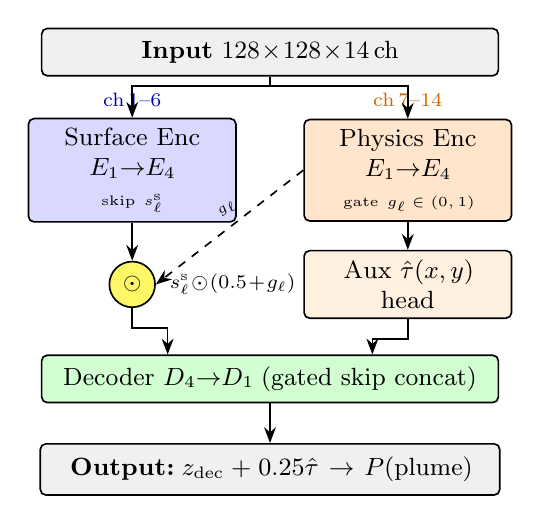
\begin{tikzpicture}[
  >=Stealth, semithick,
  B/.style={draw, rounded corners=2pt, fill=#1, align=center, font=\small},
]
%--- INPUT ---
\node[B=gray!12, minimum width=5.8cm, minimum height=0.6cm]
  (inp) at (0,6.2)
  {\textbf{Input} $128\!\times\!128\!\times\!14$\,ch};

%--- BRANCH LABELS ---
\node[font=\scriptsize, text=blue!70!black]   at (-1.75,5.6) {ch\,1--6};
\node[font=\scriptsize, text=orange!80!black] at ( 1.75,5.6) {ch\,7--14};

%--- ENCODERS ---
\node[B=blue!15, minimum width=2.6cm, minimum height=1.05cm, text width=2.4cm]
  (SE) at (-1.75,4.7)
  {Surface Enc\\$E_1{\to}E_4$\\{\tiny skip $s^\text{s}_\ell$}};
\node[B=orange!20, minimum width=2.6cm, minimum height=1.05cm, text width=2.4cm]
  (PE) at (1.75,4.7)
  {Physics Enc\\$E_1{\to}E_4$\\{\tiny gate $g_\ell\!\in\!(0,1)$}};

%--- PHYSICS GATE (below Surface Enc) ---
\node[draw, circle, fill=yellow!60, minimum size=0.58cm, inner sep=0pt, font=\footnotesize]
  (G) at (-1.75,3.25) {$\odot$};
\node[font=\scriptsize, anchor=west] at (-1.4,3.25)
  {$s^\text{s}_\ell\!\odot\!(0.5\!+\!g_\ell)$};

%--- AUX TAU HEAD ---
\node[B=orange!12, minimum width=2.6cm, minimum height=0.62cm, text width=2.4cm]
  (AUX) at (1.75,3.25)
  {Aux $\hat\tau(x,y)$ head};

%--- DECODER ---
\node[B=green!18, minimum width=5.8cm, minimum height=0.6cm]
  (DEC) at (0,2.05)
  {Decoder $D_4{\to}D_1$\;(gated skip concat)};

%--- OUTPUT ---
\node[B=gray!12, minimum width=5.8cm, minimum height=0.65cm, text width=5.6cm]
  (OUT) at (0,0.9)
  {\textbf{Output:}\;$z_\mathrm{dec}+0.25\hat\tau\to P(\text{plume})$};

%--- ARROWS ---
\draw[->] (inp.south) -- ++(0,-0.12) -| (SE.north);
\draw[->] (inp.south) -- ++(0,-0.12) -| (PE.north);
\draw[->] (SE.south) -- (G.north);
\draw[->, dashed] (PE.west)
  -- node[pos=0.45, above, font=\tiny, sloped]{$g_\ell$} (G.east);
\draw[->] (PE.south) -- (AUX.north);
\draw[->] (G.south)   -- ++(0,-0.25) -| ([xshift=-1.3cm]DEC.north);
\draw[->] (AUX.south) -- ++(0,-0.25) -| ([xshift= 1.3cm]DEC.north);
\draw[->] (DEC.south) -- (OUT.north);
\end{tikzpicture}
\caption{PhysTAUNet dual-branch architecture. The 14-channel input is split into surface channels (brightness, NDVI, reflectance) and physics channels (SWIR ratios, residual, $\Delta$-features). At each encoder level $\ell$, the Physics Encoder produces a learned sigmoid gate $g_\ell\in(0,1)$ that modulates the corresponding Surface Encoder skip connection (Eq.~\ref{eq:physgate}) before Decoder concatenation. A lightweight auxiliary head derives $\hat\tau(x,y)$ from the Physics Encoder bottleneck and adds it to the final logits (Eq.~\ref{eq:auxhead}).}
\label{fig:phystaunet}
\end{figure}

\FloatBarrier
\subsection{Loss function}

All models are trained with an identical combined binary cross-entropy and soft-Dice loss with adaptive per-sample positive-class weighting. For a sample with $n_{\text{pos}}$ and $n_{\text{neg}}$ positive and negative target pixels respectively,
\begin{equation}
w_{\text{pos}} = \operatorname{clamp}\!\left(\sqrt{\frac{n_{\text{neg}}}{n_{\text{pos}}}},\ 1.0,\ 35.0\right),
\label{eq:posweight}
\end{equation}
\begin{equation}
\mathcal{L}_{\text{BCE}} = -\frac{1}{N}\sum_i \Big[w_{\text{pos}}\,y_i\log \hat y_i + (1-y_i)\log(1-\hat y_i)\Big],
\label{eq:bce}
\end{equation}
\begin{equation}
\mathcal{L}_{\text{Dice}} = 1 - \frac{2\sum_i y_i \hat y_i + \delta}{\sum_i y_i + \sum_i \hat y_i + \delta},
\label{eq:dice}
\end{equation}
\begin{equation}
\mathcal{L} = \mathcal{L}_{\text{BCE}} + \mathcal{L}_{\text{Dice}},
\label{eq:totalloss}
\end{equation}
where $y_i$ is the (possibly soft) target, $\hat y_i$ the predicted probability, and $\delta$ a small smoothing constant in Equation~\eqref{eq:dice}. The clamp in Equation~\eqref{eq:posweight} prevents the rare, near-empty-plume patches that survive the area-fraction rejection sampling of Section~\ref{sec:plumegen} from producing degenerate, unstable gradients.

\subsection{Training protocol}

All five models are optimized with AdamW \citep{loshchilov2019decoupled} using identical learning rate and weight decay, an identical $128\times128$ patch size, an identical number of patches sampled per epoch (8192), an identical batch size (8), and an identical maximum epoch budget (40), with the best checkpoint per model selected by validation F1. Patch sampling draws rows from the background pool with a per-row sampling weight, crops a random patch from the chosen chip, and generates a fresh plume field and $\tau_0$ draw independently for every patch, so no two training patches (within or across epochs) are guaranteed identical even when drawn from the same background chip.

\subsection{Evaluation protocol}

Two metric families are reported. \emph{Strict} metrics compare predicted and target masks pixel-for-pixel after thresholding predictions at $0.5$: precision, recall, F1, intersection-over-union (IoU), and overall accuracy. \emph{Tolerant} metrics apply a 2-pixel morphological dilation to both predicted and target masks before scoring, following standard practice in boundary-sensitive segmentation evaluation, to separate genuine detection failures from sub-pixel boundary disagreement. All metrics are computed identically for VAL (used for checkpoint selection) and for a held-out synthetic TEST split whose background chips were not used in training or in checkpoint selection for any model.

\subsection{Inference efficiency benchmarking}

Parameter count, checkpoint size, approximate GFLOPs per image (counting convolution, transposed-convolution, and linear-layer operations only; batch normalization, activations, pooling, and interpolation are excluded, so figures should be read as an architecture-comparison estimate rather than an exact hardware trace), and forward-pass latency are measured on the held-out TEST split using the same synthetic injection settings as evaluation. Reported latency is model-only: input batches are fully prepared (synthetic plume generation and feature stacking complete) before timing begins, so data loading and plume generation cost are excluded from the reported numbers by design, and should be added separately when estimating end-to-end deployment latency.

\section{Experimental Protocol and Fairness Statement}
\label{sec:protocol}

To isolate the effect of architecture from every other variable, all five models in this benchmark share: the identical 14-channel input representation (Section~\ref{sec:features}); the identical synthetic plume generator, injection procedure, and target construction (Sections~\ref{sec:plumegen}--\ref{sec:injection}); the identical combined BCE+Dice loss with identical positive-weight clamping (Equations~\eqref{eq:posweight}--\eqref{eq:totalloss}); the identical AdamW optimizer configuration, learning rate, weight decay, batch size, patch size, and patches-per-epoch budget; the identical background chip pool and deterministic TRAIN/VAL/TEST split produced by spatial blocking; and identical checkpoint-selection-by-validation-F1 and held-out TEST evaluation procedures. The only varying factor across the five runs is the architecture itself (Section~\ref{sec:architectures}). Each model was trained for a single run with a fixed random seed; we did not perform multi-seed repetition, a limitation discussed in Section~\ref{sec:discussion}.

\FloatBarrier
\section{Results}
\label{sec:results}

\begin{table*}[t]
\centering
\caption{Segmentation accuracy on the controlled synthetic benchmark, validation (VAL) and held-out synthetic test (TEST) splits. Models are ranked by TEST F1. Tolerant metrics use a 2-pixel boundary dilation. Bold marks the best value per column.}
\label{tab:main_results}
\small
\begin{tabular}{l ccccc ccccc}
\toprule
 & \multicolumn{5}{c}{VAL} & \multicolumn{5}{c}{TEST} \\
\cmidrule(lr){2-6} \cmidrule(lr){7-11}
Model & F1 & IoU & Prec. & Rec. & Tol.\,F1 & F1 & IoU & Prec. & Rec. & Tol.\,F1 \\
\midrule
Attention U-Net & \textbf{0.461} & \textbf{0.300} & 0.442 & 0.482 & \textbf{0.588} & \textbf{0.455} & \textbf{0.294} & 0.442 & 0.469 & \textbf{0.577} \\
DeepLabV3+ & 0.439 & 0.281 & \textbf{0.474} & 0.409 & 0.556 & 0.445 & 0.286 & \textbf{0.484} & 0.411 & 0.557 \\
U-Net & 0.451 & 0.291 & 0.384 & \textbf{0.546} & 0.581 & 0.437 & 0.280 & 0.377 & \textbf{0.520} & 0.560 \\
PhysTAUNet & 0.448 & 0.289 & 0.405 & 0.502 & 0.570 & 0.436 & 0.278 & 0.386 & 0.500 & 0.551 \\
U-Net++ & 0.443 & 0.285 & 0.409 & 0.484 & 0.563 & 0.419 & 0.265 & 0.388 & 0.455 & 0.534 \\
\bottomrule
\end{tabular}
\end{table*}


Table~\ref{tab:main_results} reports strict and tolerant segmentation accuracy on VAL and TEST, ranked by TEST F1. On VAL, Attention U-Net is the strongest model on F1 (0.461), IoU (0.300), and tolerant F1 (0.588); U-Net is second on F1 (0.451) but has the highest recall (0.546) and lowest precision (0.384) of all five models, consistent with the over-prediction behavior discussed below. DeepLabV3+ ranks fourth on VAL F1 (0.439) despite having the highest precision (0.474) of any model, indicating a conservative decision boundary rather than a weak feature representation.

On TEST, Attention U-Net remains the strongest model (F1 = 0.455, IoU = 0.294), but the remaining ranking reshuffles: DeepLabV3+ rises from fourth on VAL to second on TEST (F1 = 0.445), overtaking both U-Net (0.437) and PhysTAUNet (0.436), while U-Net++ falls to last on TEST (F1 = 0.419) after ranking fourth on VAL. PhysTAUNet is fourth of five on both VAL and TEST. Figure~\ref{fig:val_metrics} and Figure~\ref{fig:test_metrics} show the corresponding strict and tolerant metric bars for VAL and TEST, and Figure~\ref{fig:pr} shows the precision--recall trade-off by model. Tolerant metrics recover an absolute $0.10$--$0.13$ F1 across every model relative to strict scoring, indicating that a substantial share of disagreement between predictions and targets is boundary-localized (within 2 pixels) rather than gross detection failure, and that this boundary effect is roughly uniform across architectures rather than concentrated in any one model.

\begin{figure*}[t]
\centering
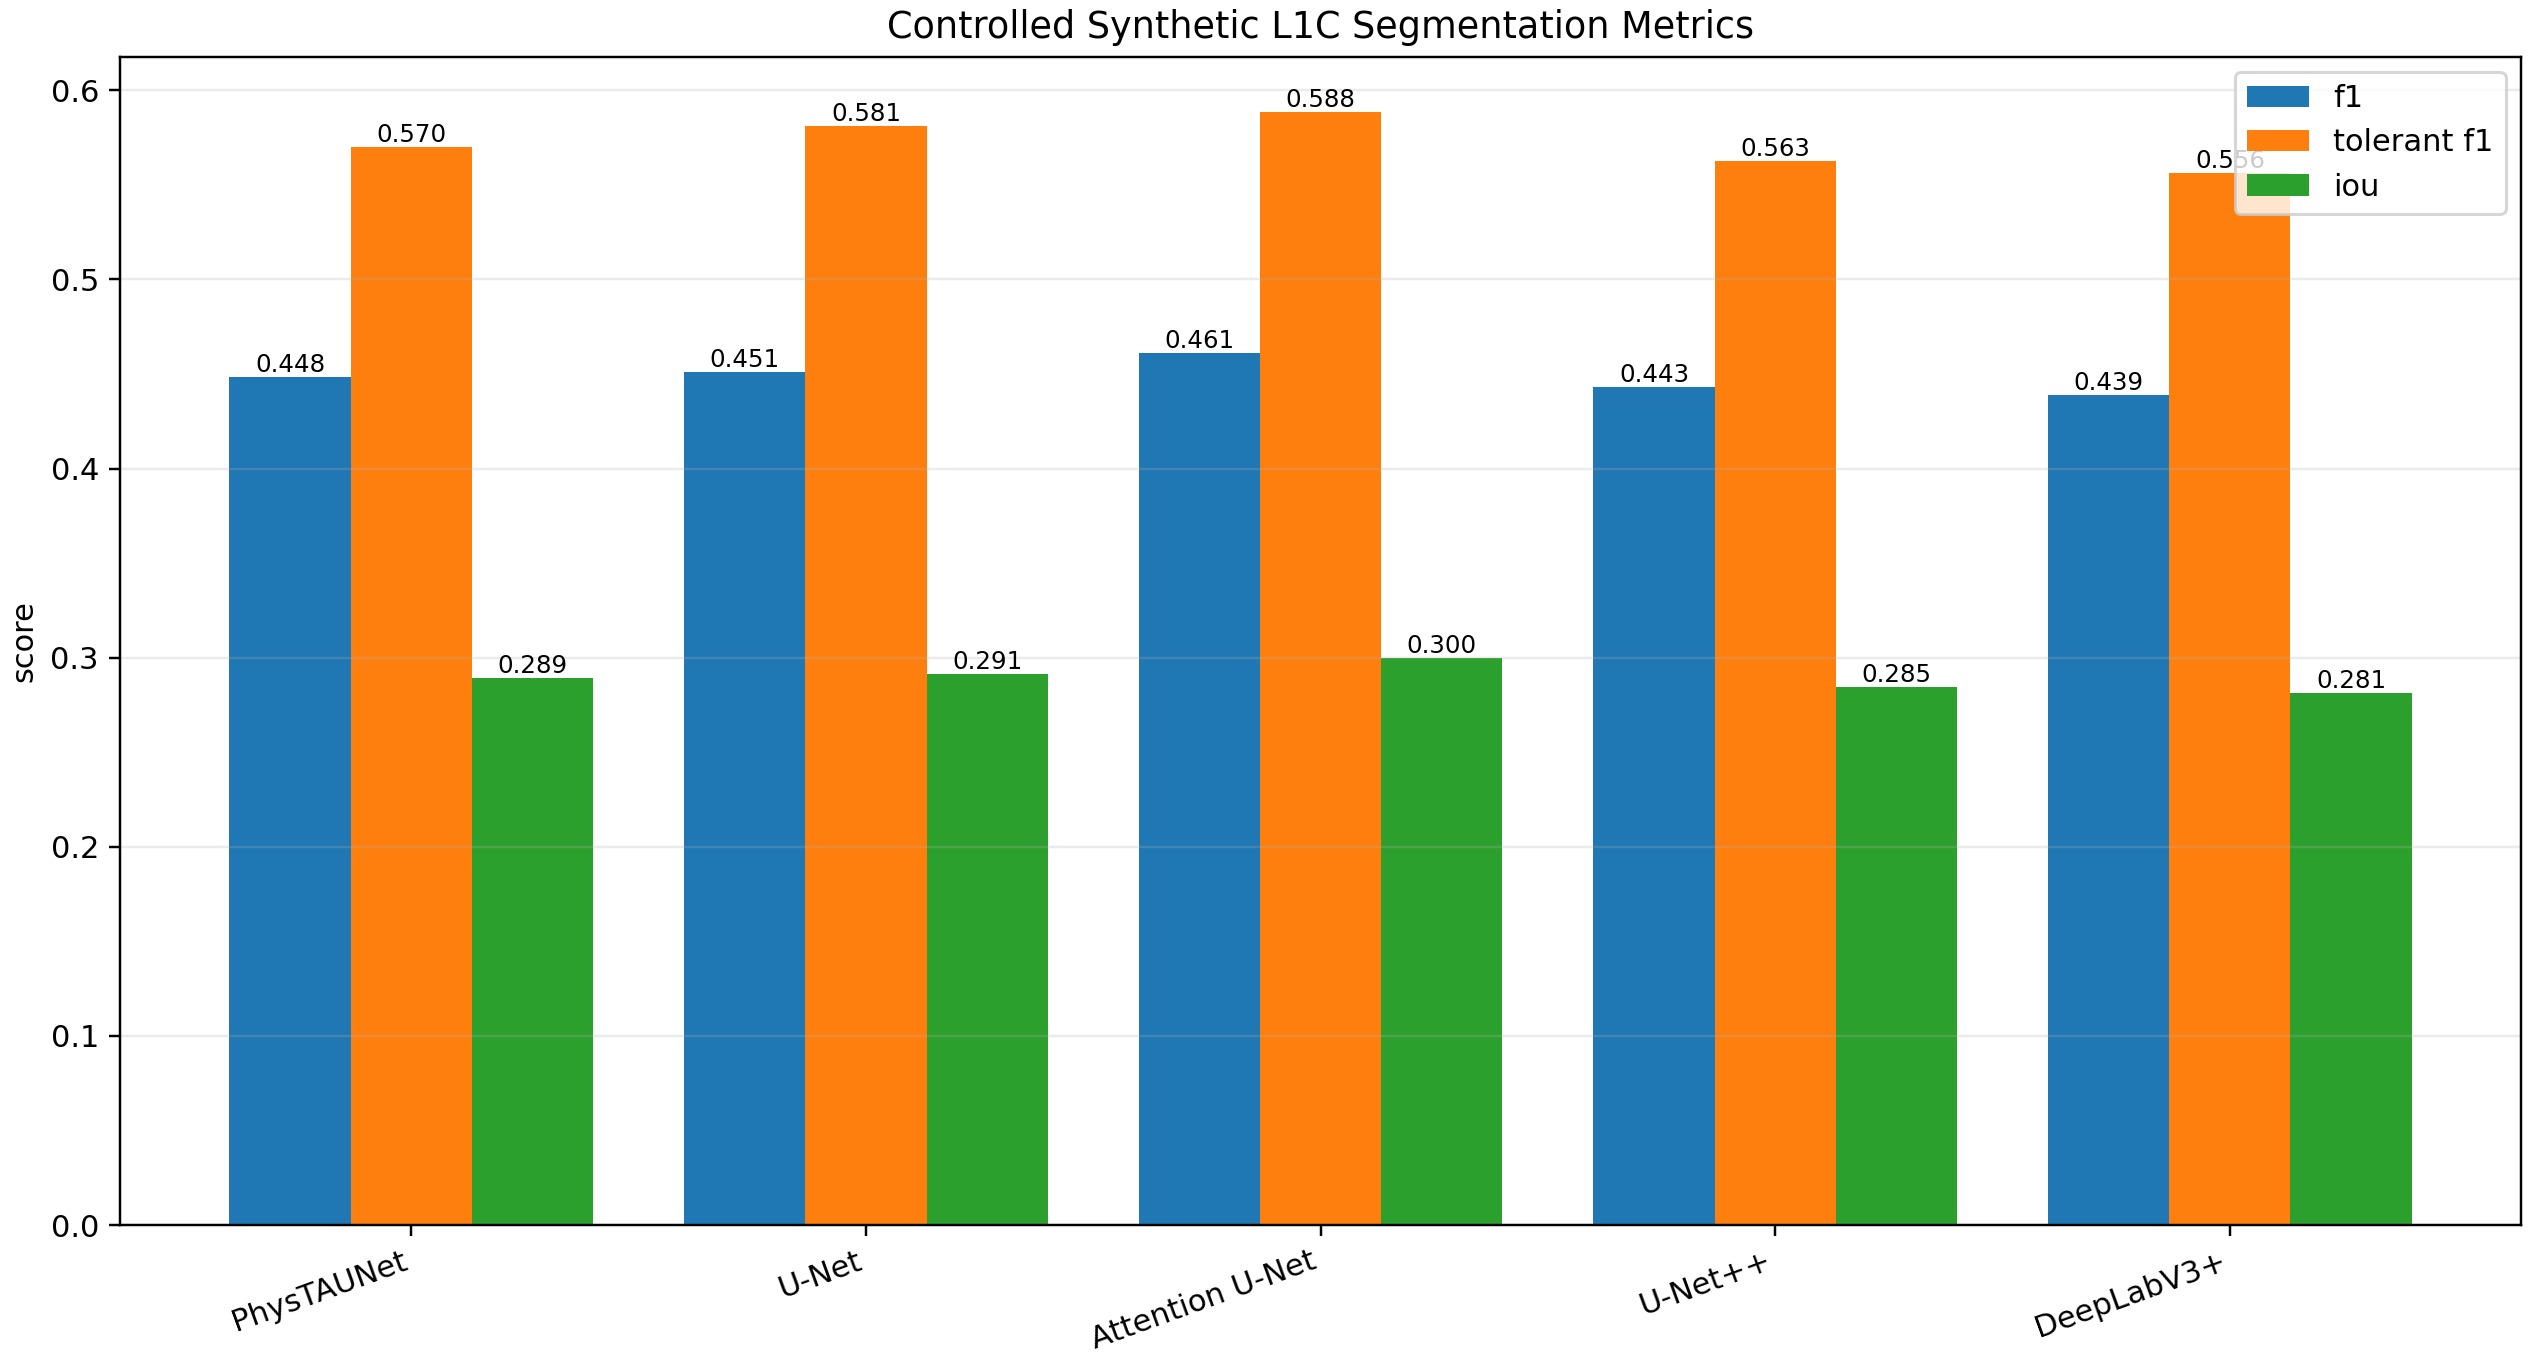
\includegraphics[width=0.92\textwidth]{figures/metrics_synthetic_segmentation.png}
\caption{Validation-split segmentation metrics (F1, IoU, accuracy, strict and tolerant) for all five benchmarked models.}
\label{fig:val_metrics}
\end{figure*}

\begin{figure*}[t]
\centering
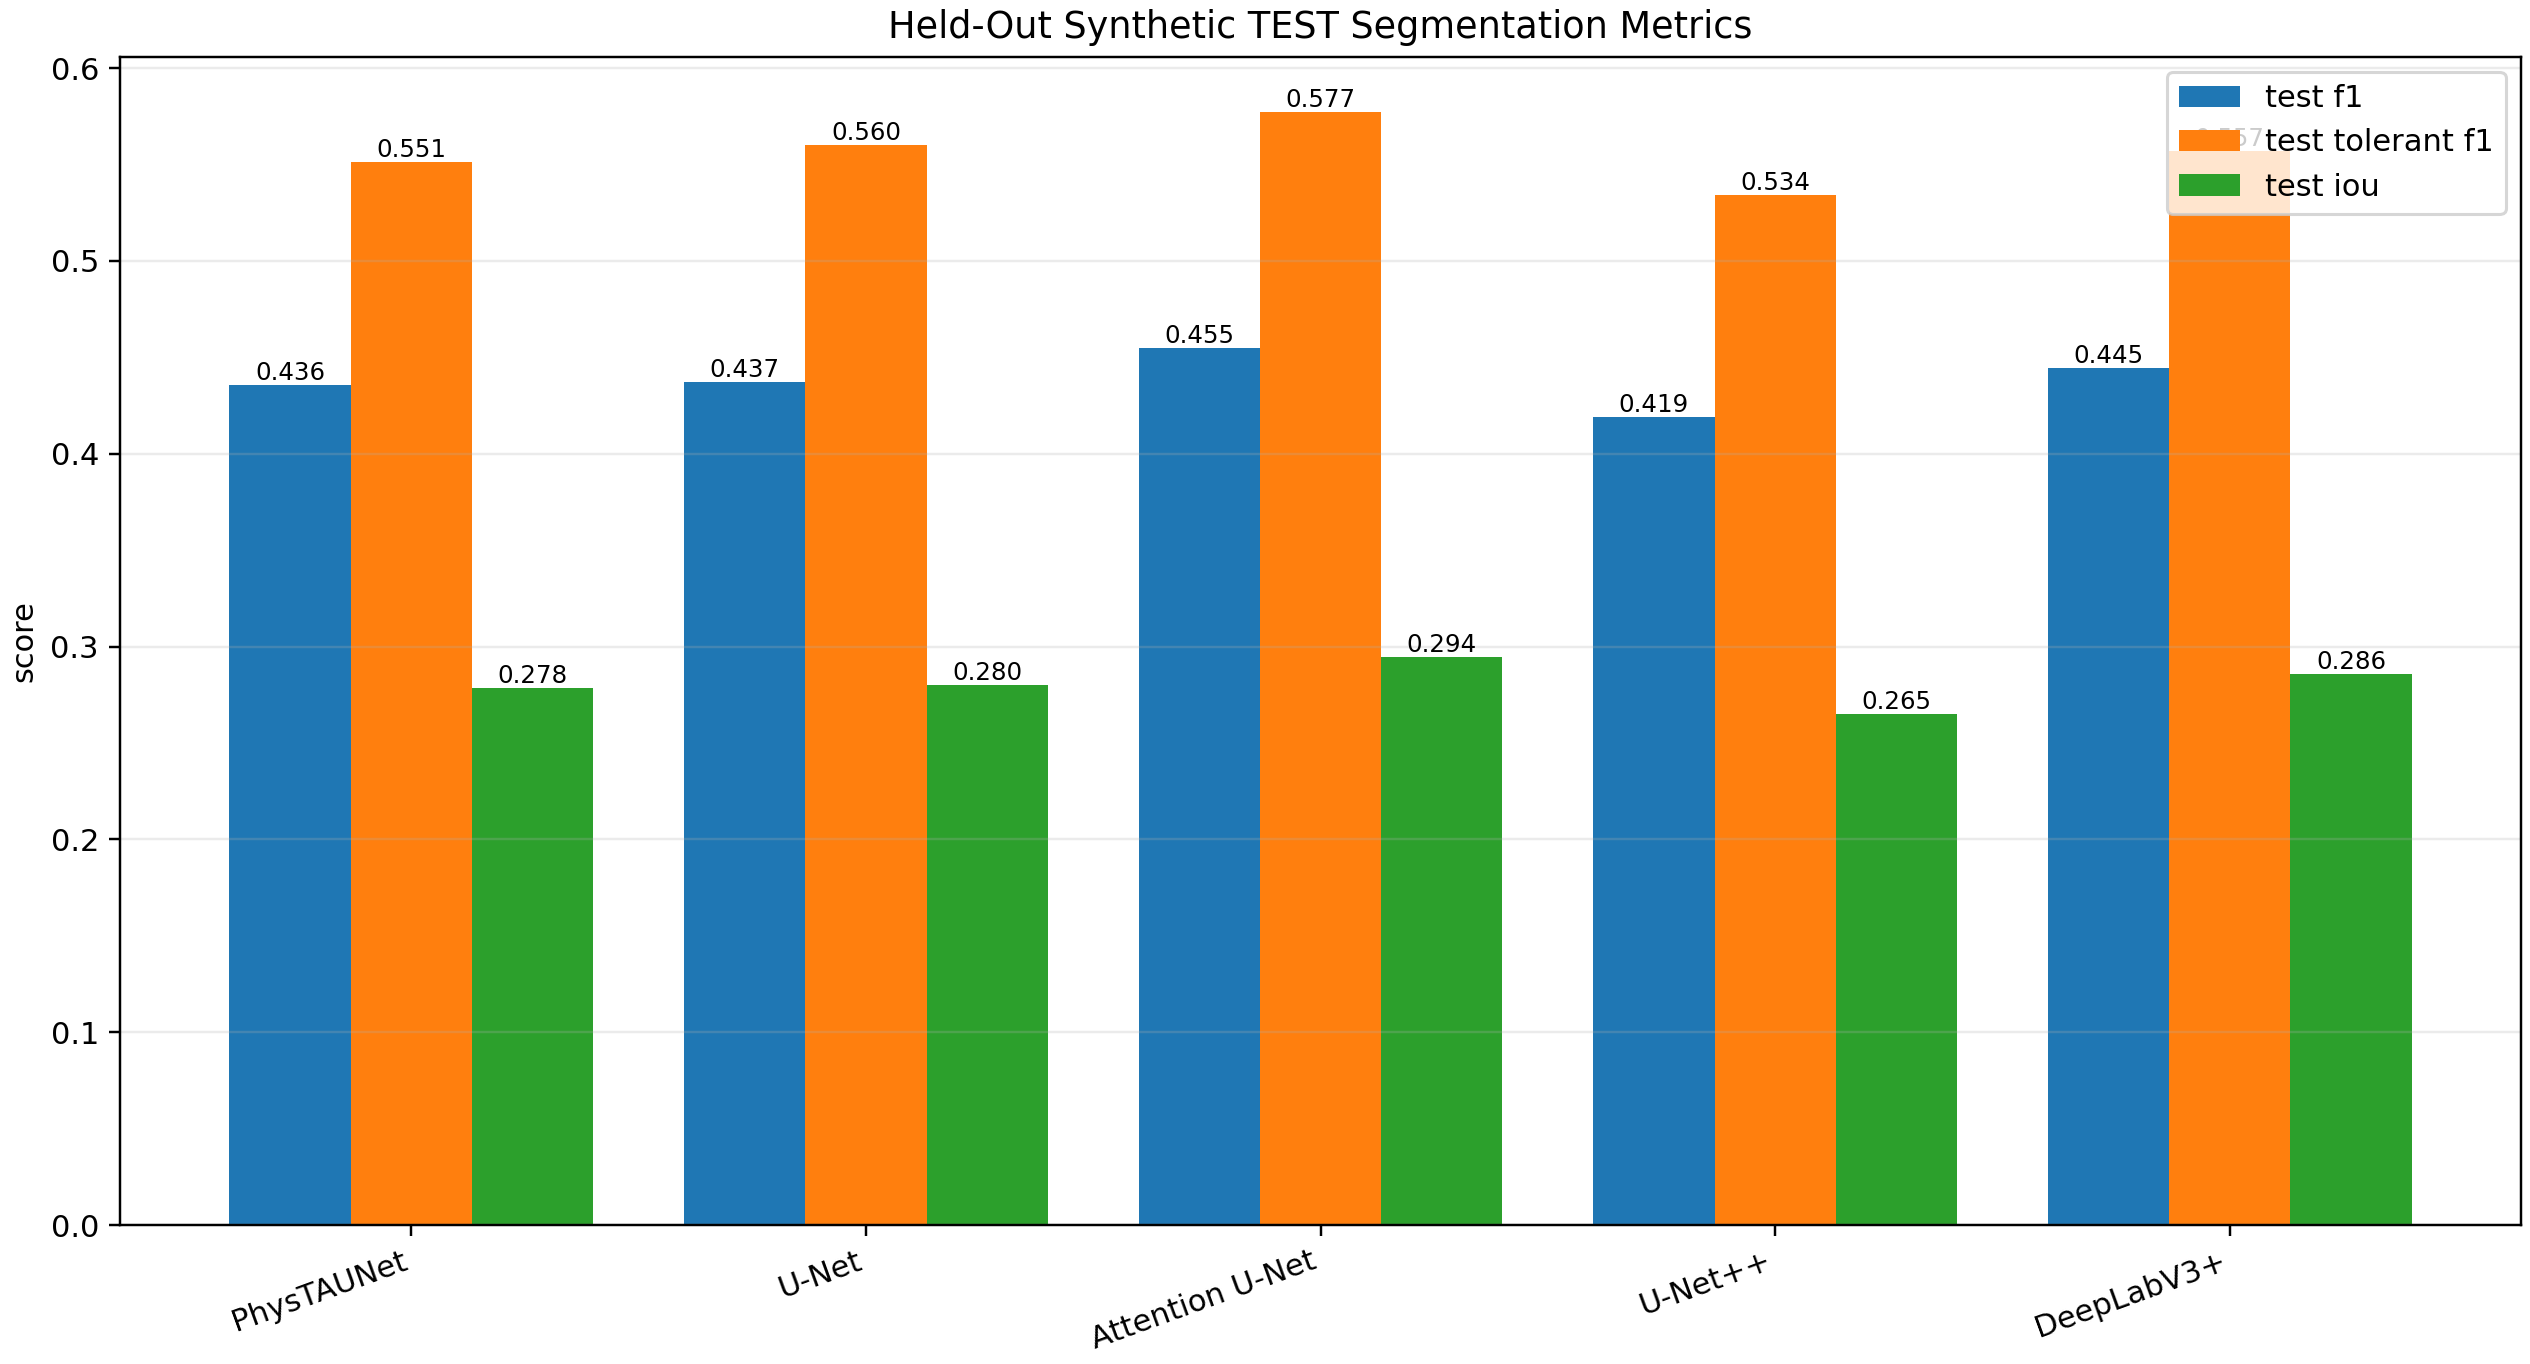
\includegraphics[width=0.92\textwidth]{figures/metrics_synthetic_test_segmentation.png}
\caption{Held-out synthetic TEST-split segmentation metrics for all five benchmarked models, computed on background chips never used during training or checkpoint selection.}
\label{fig:test_metrics}
\end{figure*}

\begin{figure*}[t]
\centering
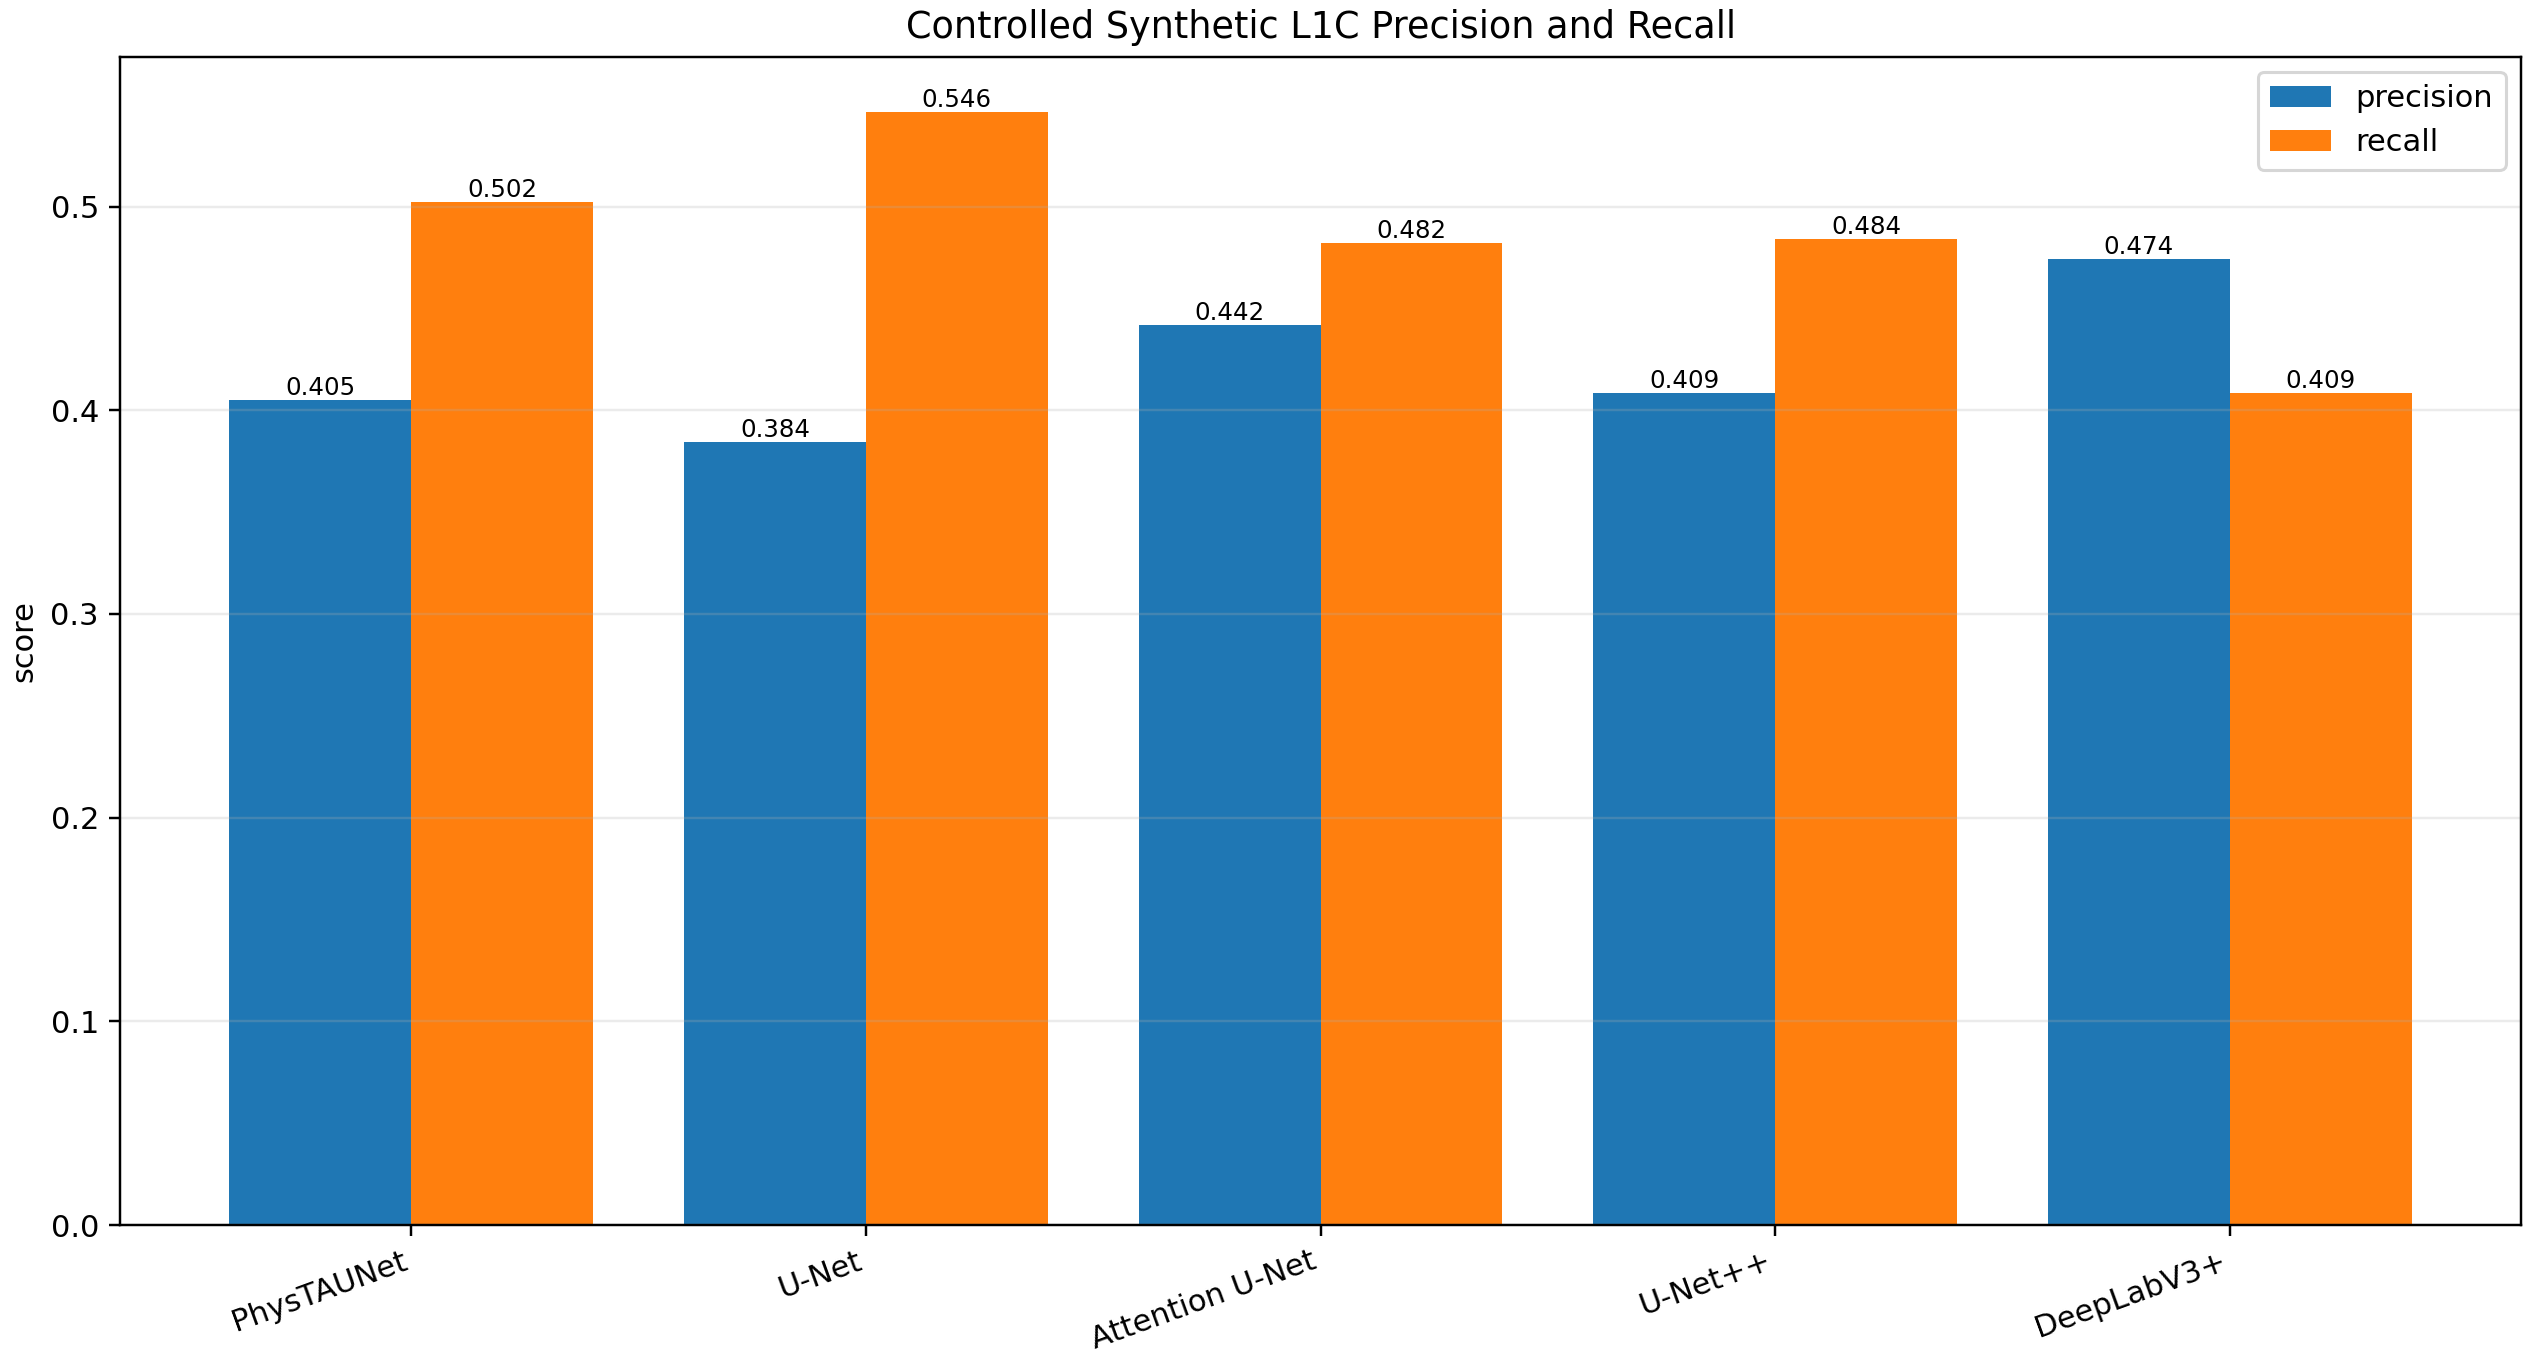
\includegraphics[width=0.92\textwidth]{figures/metrics_synthetic_precision_recall.png}
\caption{Precision and recall by model. DeepLabV3+ is the most conservative (highest precision, lowest recall); U-Net is the most liberal (lowest precision, highest recall).}
\label{fig:pr}
\end{figure*}

The predicted positive-pixel fraction is informative alongside precision/recall: the true mean positive fraction is $8.3\%$ (VAL) and $8.2\%$ (TEST) for every model, since all models share the same target distribution by construction, yet predicted positive fractions range from $7.0\%$ (DeepLabV3+, under-predicting plume extent) to $11.8\%$ (U-Net, over-predicting). PhysTAUNet's predicted fraction ($10.3\%$ VAL, $10.6\%$ TEST) is closer to U-Net's over-prediction tendency than to Attention U-Net's near-calibrated fraction ($9.1\%$ VAL, $8.7\%$ TEST), suggesting Attention U-Net's gating mechanism specifically improves calibration of predicted plume extent rather than only improving raw pixel accuracy.

\subsection{Qualitative results}

Figure~\ref{fig:qual1} shows a representative example comparing all five models' predicted probability maps against the RGB composite, the SWIR ratio delta, and the ground-truth mask for one held-out TEST patch; the remaining five qualitative examples are provided in the Supplementary Material. Across examples, all models correctly localize the plume core but disagree most at the diffuse, low-optical-depth periphery and at detached wisp regions (Section~\ref{sec:plumegen}), consistent with the boundary-driven gap between strict and tolerant metrics in Table~\ref{tab:main_results}.

\begin{figure*}[t]
\centering
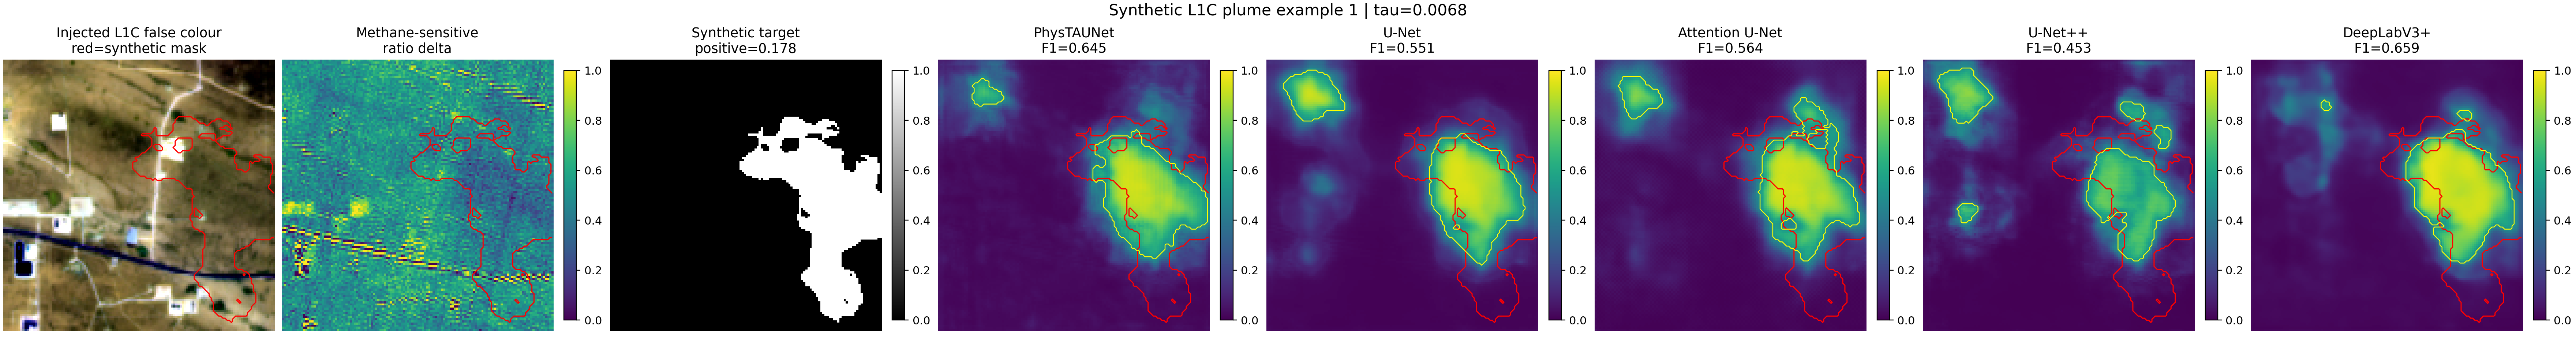
\includegraphics[width=\textwidth]{figures/synthetic_example_01_model_comparison.png}
\caption{Representative qualitative comparison: RGB composite, SWIR ratio delta, ground-truth soft target, and per-model predicted probability maps for one held-out TEST patch. Additional examples are provided in the Supplementary Material (Figures S1--S5).}
\label{fig:qual1}
\end{figure*}

\subsection{Inference efficiency}

\begin{table*}[t]
\centering
\caption{Inference efficiency on held-out synthetic TEST patches ($128\times128$, batch size 8, CUDA). Latency is model-only forward pass (data loading and plume generation excluded). GFLOPs/image counts convolution, transposed-convolution, and linear-layer operations only. Models are ranked by median latency.}
\label{tab:efficiency}
\small
\begin{tabular}{lccccc}
\toprule
Model & Params (M) & GFLOPs/img & p50 (ms) & img/s & TFLOPs \\
\midrule
U-Net & 1.93 & 5.32 & 0.573 & 1839 & 9.78 \\
U-Net++ & 1.93 & 5.46 & 0.592 & 1923 & 10.51 \\
Attention U-Net & 1.97 & 5.52 & 0.616 & 1405 & 7.75 \\
DeepLabV3+ & 1.33 & 11.46 & 0.662 & 1507 & 17.26 \\
PhysTAUNet & 3.75 & 6.61 & 0.882 & 1173 & 7.76 \\
\bottomrule
\end{tabular}
\end{table*}


Table~\ref{tab:efficiency} and Figure~\ref{fig:efficiency} report parameter count, estimated GFLOPs per image, and forward-pass latency/throughput on TEST. U-Net and U-Net++ are the smallest and fastest models (1.93M parameters, $\geq$1838 images/s). DeepLabV3+ has the fewest parameters (1.33M) but the highest compute density (11.46 GFLOPs/image, 17.26 effective TFLOPs achieved) owing to its dilated-convolution ASPP module, and a mid-pack throughput (1507 images/s). PhysTAUNet is the largest model by a wide margin (3.75M parameters, roughly $1.9\times$ Attention U-Net and $1.9$--$2\times$ the other four models) and has the lowest throughput of all five (1173 images/s) and the highest median latency (0.882 ms/image versus 0.573--0.662 ms for the other four), a direct consequence of its dual-branch encoder and auxiliary head.

\begin{figure*}[t]
\centering
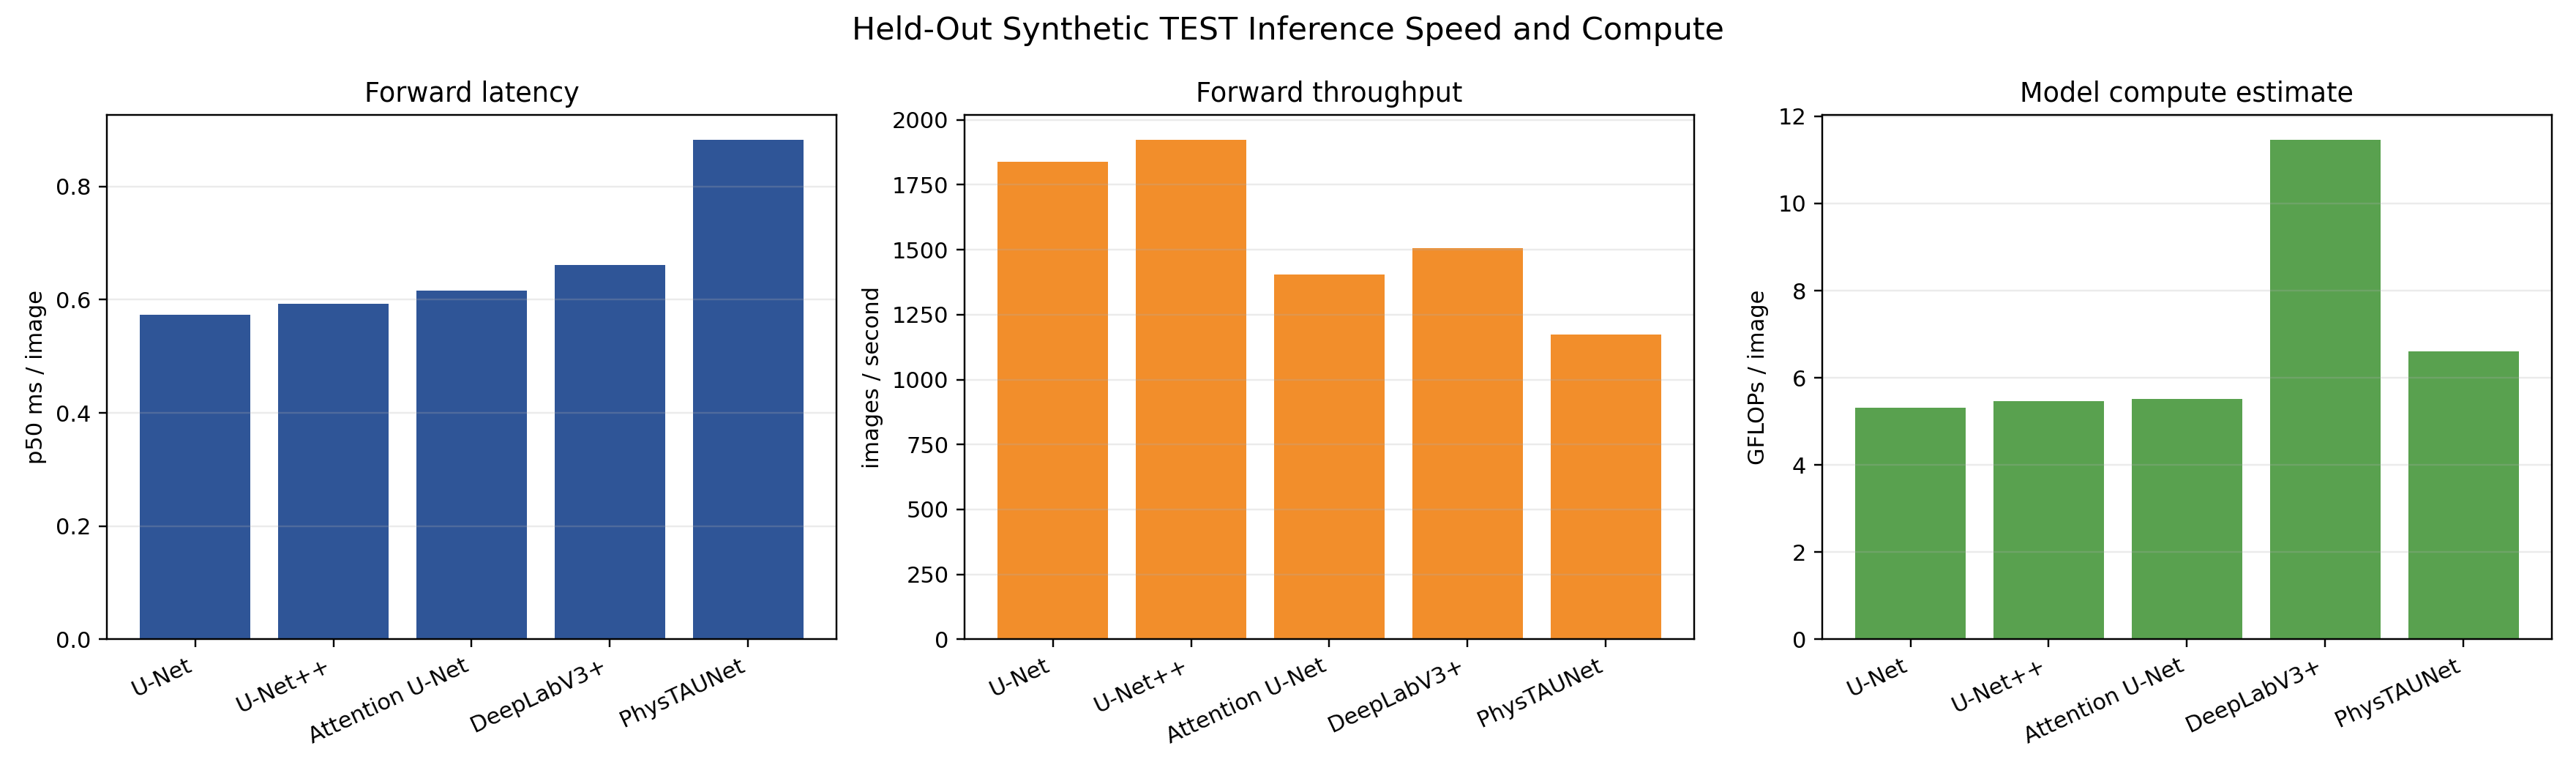
\includegraphics[width=0.92\textwidth]{figures/inference_speed_gflops_test.png}
\caption{Inference efficiency on held-out TEST patches: parameter count, GFLOPs/image, and throughput by model.}
\label{fig:efficiency}
\end{figure*}

Combining Tables~\ref{tab:main_results} and~\ref{tab:efficiency}: the most accurate model in this benchmark (Attention U-Net) is not the most expensive, ranking third of five on parameter count and median latency; the most expensive and slowest model (PhysTAUNet) is not the most accurate, ranking fourth of five on TEST F1. We treat this as the central empirical finding of the benchmark and discuss its implications in Section~\ref{sec:discussion}.

\clearpage
\section{Discussion}
\label{sec:discussion}

The three subsections below interpret the benchmark's four empirical findings in sequence: why the lightweight Attention U-Net gate leads on both VAL and TEST despite simpler architecture (Section~\ref{sec:disc_attn}), why DeepLabV3+ rises from fourth to second between splits (Section~\ref{sec:disc_deep}), and what the auxiliary optical-depth head in PhysTAUNet does and does not demonstrate in this controlled setting (Section~\ref{sec:disc_phys}). Section~\ref{sec:limitations} then catalogues five limitations that bound how the results should be read.

\subsection{Why attention gating outperforms physics gating here}
\label{sec:disc_attn}

Attention U-Net's advantage over the other four models is small in absolute terms (TEST F1 0.455 versus 0.436--0.445) but consistent across both VAL and TEST and across strict and tolerant scoring, and it is achieved with a comparatively cheap architectural addition: a sigmoid gate computed from the decoder's own bottleneck-derived state, applied to the existing skip connections, with no additional encoder branch. We hypothesize this end-to-end-learned, single-branch gate generalizes better than PhysTAUNet's fixed two-branch channel routing for two reasons specific to this benchmark's construction. First, the injected physics is a single mechanism (Equation~\eqref{eq:beerlambert} acting on one band), so the eight engineered features of Section~\ref{sec:features} already make the relevant signal close to linearly separable from background texture; a learned attention gate can exploit this directly from the full 14-channel input without needing a dedicated encoder branch to isolate it. Second, PhysTAUNet's hard channel partition into ``surface'' and ``physics'' branches (Section~\ref{sec:architectures}) is a design-time assumption about which channels carry physical signal; if that partition is even mildly suboptimal, the gain from explicit physics-routing may not offset the cost of a larger, harder-to-optimize parameter space (3.75M parameters against 1.97M for Attention U-Net) under a fixed 40-epoch budget.

\subsection{Why DeepLabV3+ rises from VAL to TEST}
\label{sec:disc_deep}

DeepLabV3+'s rank-four-to-rank-two shift between VAL and TEST (Table~\ref{tab:main_results}) is the largest rank change of any model and is consistent with its precision-dominant, recall-conservative behavior: its dilated-convolution ASPP module aggregates context at multiple fixed scales, which may generalize more robustly to the freshly sampled plume sizes and positions of the TEST split's independent synthetic draws than the single-scale skip connections of the U-Net family. We note this as a plausible mechanistic hypothesis rather than a settled explanation, since the rank shift, while consistent in direction across strict and tolerant metrics, is based on a single training run per model (Section~\ref{sec:protocol}) and could in part reflect run-to-run variance rather than a stable generalization property of dilated convolutions.

\subsection{What PhysTAUNet's auxiliary head does and does not demonstrate}
\label{sec:disc_phys}

PhysTAUNet's auxiliary optical-depth head (Equation~\eqref{eq:auxhead}) is not supervised against the true field $\tau_0\tau(x,y)$ and therefore cannot be evaluated as a calibrated retrieval in this benchmark; its only training signal is the downstream segmentation loss. The architecture's contribution in its current form is structural interpretability: it exposes an explicit, inspectable physics pathway through the network, rather than a demonstrated accuracy or efficiency advantage; on this controlled benchmark it is outperformed on every accuracy metric in Table~\ref{tab:main_results} by at least one simpler, cheaper baseline. We consider it an open and testable hypothesis, not yet supported by the present results, that physics-gated routing would show a clearer advantage under conditions this controlled benchmark does not include by design: multiple co-occurring physical mechanisms (e.g., aerosol scattering or surface-reflectance confounds in addition to SWIR absorption), or genuine real-sensor domain shift between training and deployment, neither of which is present when the only injected signal is a single Beer--Lambert mechanism shared identically across train, validation, and test.

\subsection{Limitations}
\label{sec:limitations}

This benchmark has five limitations that bound how its results should be read. First, the injected physics is restricted to single-band Beer--Lambert attenuation of $B12$; it does not model atmospheric scattering, aerosol interaction, cloud or cloud-shadow confounds \citep{ulmer2025deep}, or multiple overlapping plumes at different heights, so architectural advantages observed here may not persist under richer physical confounds. Second, the 2-pixel tolerant-metric dilation (Section~\ref{sec:results}) recovers a large, roughly uniform F1 gain across all models; this indicates boundary disagreement dominates strict-metric gaps, but the specific tolerance radius was not itself ablated, and a different radius could compress or widen the gaps between models. Third, each model was trained once, with one fixed seed (Section~\ref{sec:protocol}); the F1 gaps separating U-Net, PhysTAUNet, and U-Net++ on VAL (0.451, 0.448, 0.443) are small enough that they plausibly fall within run-to-run variance, and the ranking among these three specifically should not be over-interpreted as a stable ordering without multi-seed repetition. Fourth, the efficiency benchmark of Section~\ref{sec:results} measures forward-pass latency only, excluding the cost of feature computation (Section~\ref{sec:features}) and, during training, plume generation (Section~\ref{sec:plumegen}); the latter is itself non-trivial and would need to be included in any end-to-end deployment latency 